
 
\subsection{Visualizing the convolution kernels} \label{sec:visualize_operator}
We begin by evaluating the functions $f, _{+2}f ~\&~ _{-2}f $. Since these functions determine the amplitude of the convolution kernels as a function of the angular distance $\beta$ from the central pixel, we refer to them as the radial kernels. These functions have been calculated by evaluating the multipole sums in \eq{eq:rad_ker_queb} and \eq{eq:rad_ker_quequbqu} from $\ell_{\rm min}=2$ to $\ell_{\rm max}=96$. The resultant functions are depicted in \fig{fig:beta_kernel}. Note that the function $f(\beta)$, which is a part of the  real space convolution  kernel which translates the coordinate dependent Stokes Q \& U to coordinate independent scalars E \& B, has a vanishing contribution from the location of the central pixel ($\beta \rightarrow 0$). 
%
\begin{figure}[!hbt]
\centering
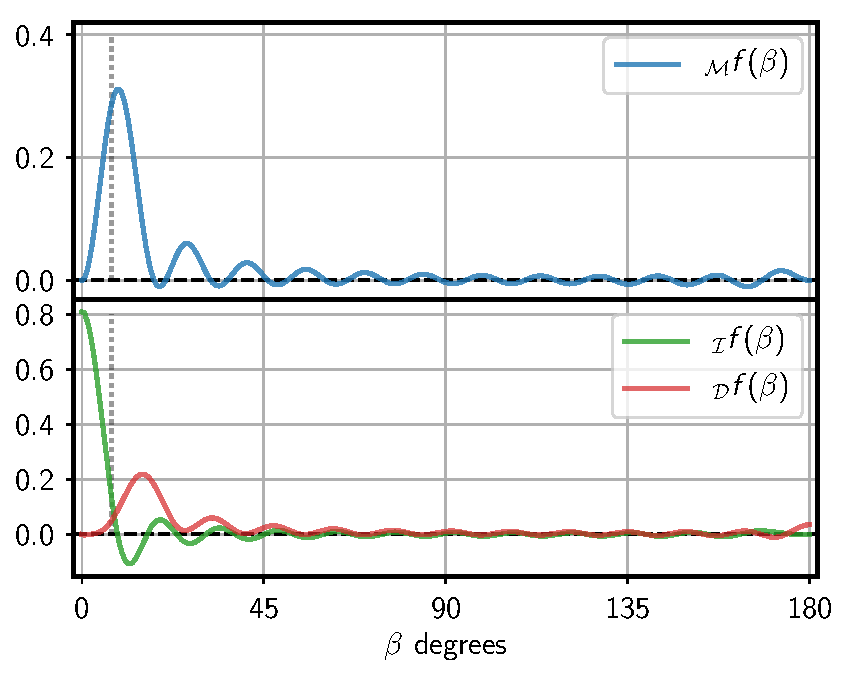
\includegraphics[width=0.8\columnwidth]{kernel/beta_kernel.pdf}
\caption{The figure depicts the radial part of the convolution kernels shown in \fig{fig:vis_kernel}. These radial function have been evaluated with the band limit fixed at $\ell_{\rm max}=96$. The vertical dashed line marks the approximate size of a NSIDE=32 Healpix pixel. \comment{Update to Nside=64 ?}}
\label{fig:beta_kernel}
\end{figure}
%
We recall that the fields E \& B are scalar and hence immune to coordinate definitions. The locally defined Stokes parameters however necessarily depend on the coordinate definition. Therefore, this nature of the radial kernel is to be expected in order for it to satisfy the requirement of the derived quantities being scalars. The functions $_{+2}f(\beta)~\&~_{-2}f(\beta)$, both contribute to the convolution kernels which decompose the Stokes parameters into those corresponding to the respective scalar modes E \& B. Note that while $_{-2}f(\beta)$ specifically contributes at the location of the central pixel, $_{+2}f(\beta)$ dominates in the neighbouring regions which are approximately at least 1 pixel away from the central pixel.

In addition to the angular distance $\beta$ from the central pixel, the convolution kernels also depend on the other Euler angles $\alpha ~\&~ \gamma$ as seen from \eq{eq:op_qu2eb}, \eq{eq:fn_i} and \eq{eq:fn_d}. We plot the real and imaginary parts of the functions $\mathcal{M}, \mathcal{D}~\&~\mathcal{I}$ at different positions on the sphere. For illustration the functions have been sampled at a very high Healpix resolution parameter of NSIDE=2048. We evaluate parts of the convolution kernels at different locations on the sphere and the results are depicted in \fig{fig:vis_kernel}. 
 %
\begin{figure}[!h] \label{fig:mixing_kernel}
\centering
%\captionsetup[subfigure]{labelformat=empty}
\subfigure{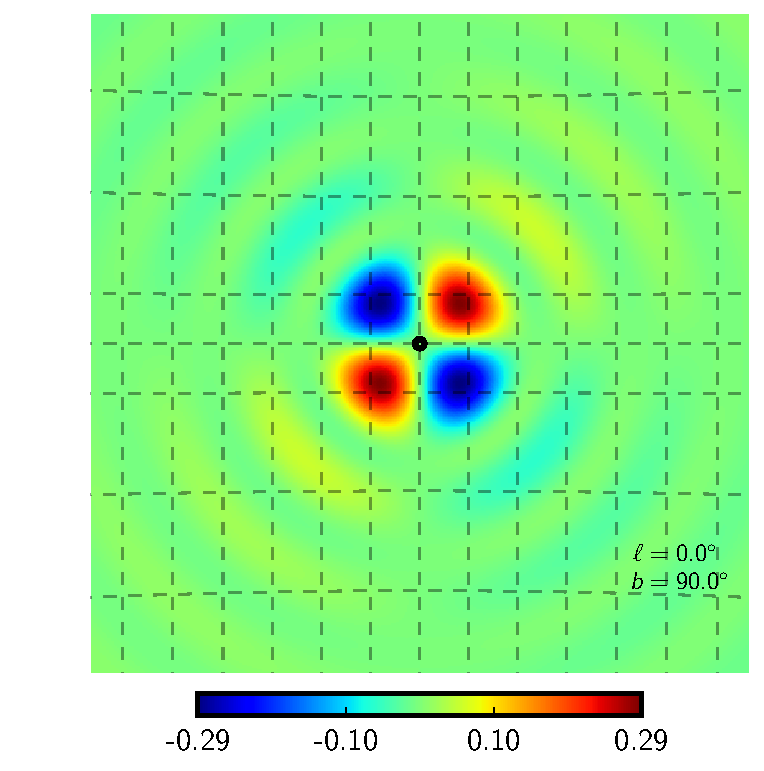
\includegraphics[width=0.16\columnwidth]{kernel/qu2eb_ker_r_lat90_lon0.pdf}}\hspace{-2mm}
\subfigure{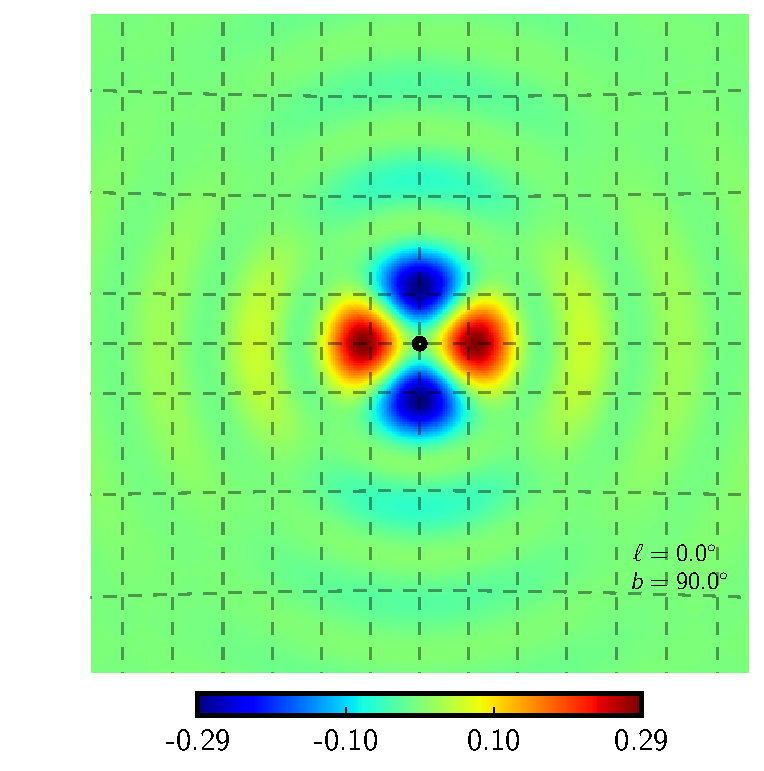
\includegraphics[width=0.16\columnwidth]{kernel/qu2eb_ker_i_lat90_lon0.pdf}}\hspace{-2mm}
\subfigure{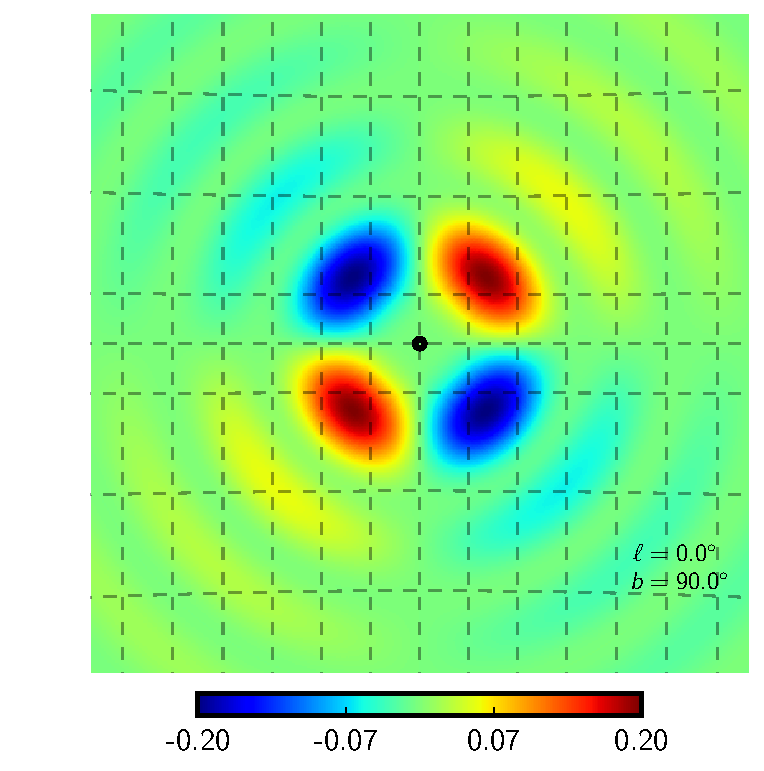
\includegraphics[width=0.16\columnwidth]{kernel/qu2ebqu_ker_r_lat90_lon0.pdf}}\hspace{-2mm}
\subfigure{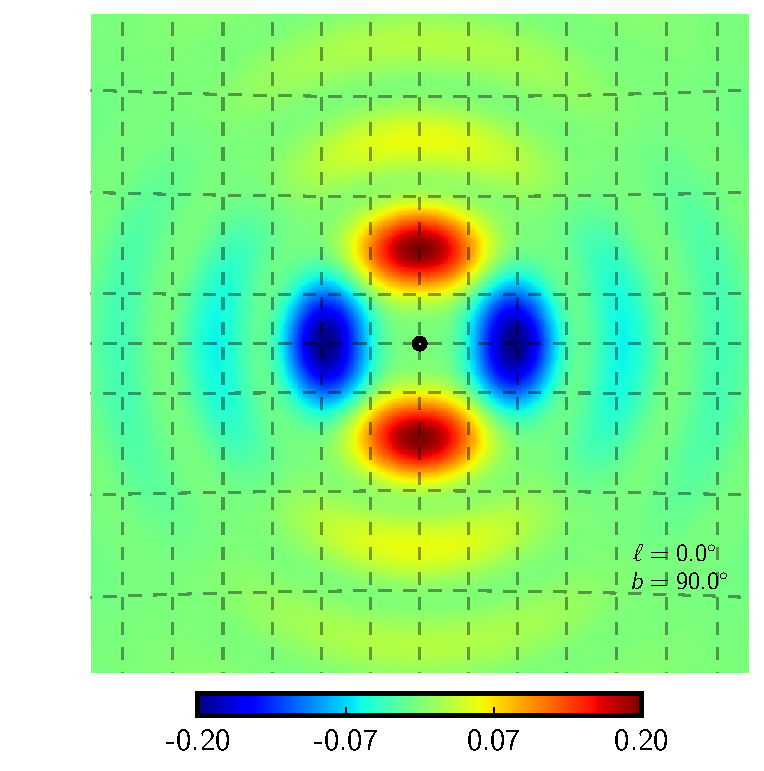
\includegraphics[width=0.16\columnwidth]{kernel/qu2ebqu_ker_i_lat90_lon0.pdf}}\hspace{-2mm}
\subfigure{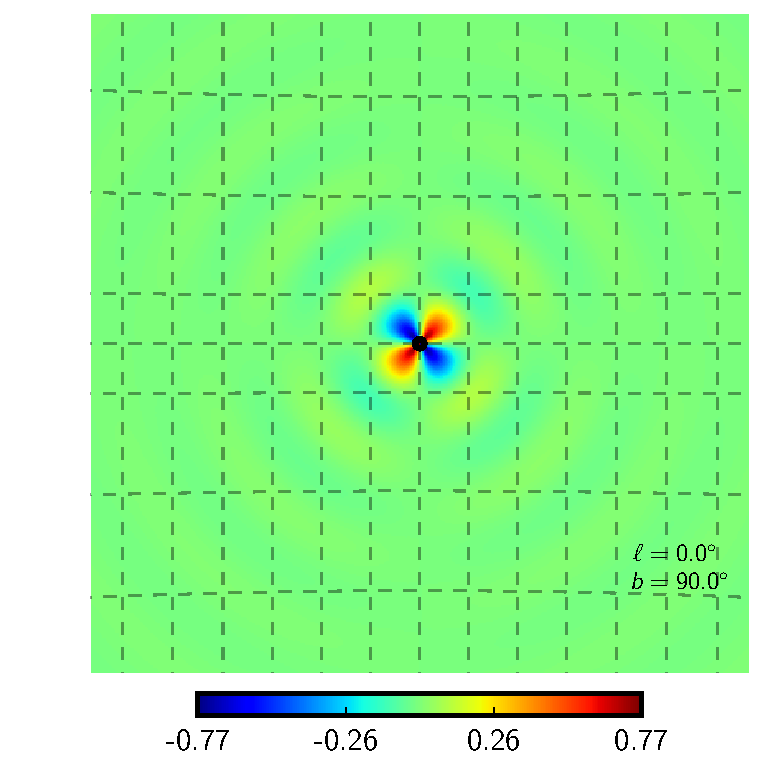
\includegraphics[width=0.16\columnwidth]{kernel/I_ker_r_lat90_lon0.pdf}}\hspace{-2mm}
\subfigure{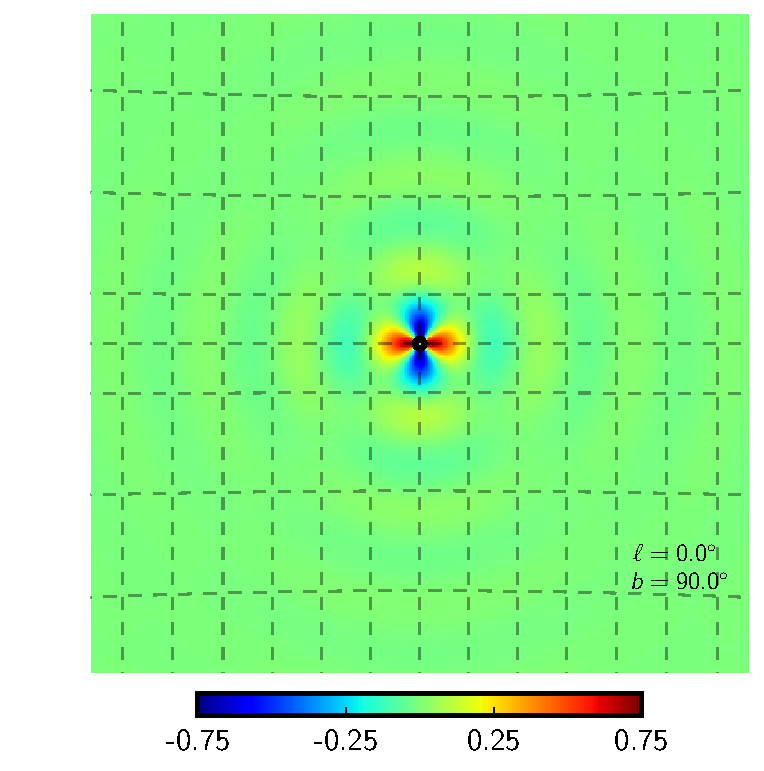
\includegraphics[width=0.16\columnwidth]{kernel/I_ker_i_lat90_lon0.pdf}}\\[-2ex]
\subfigure{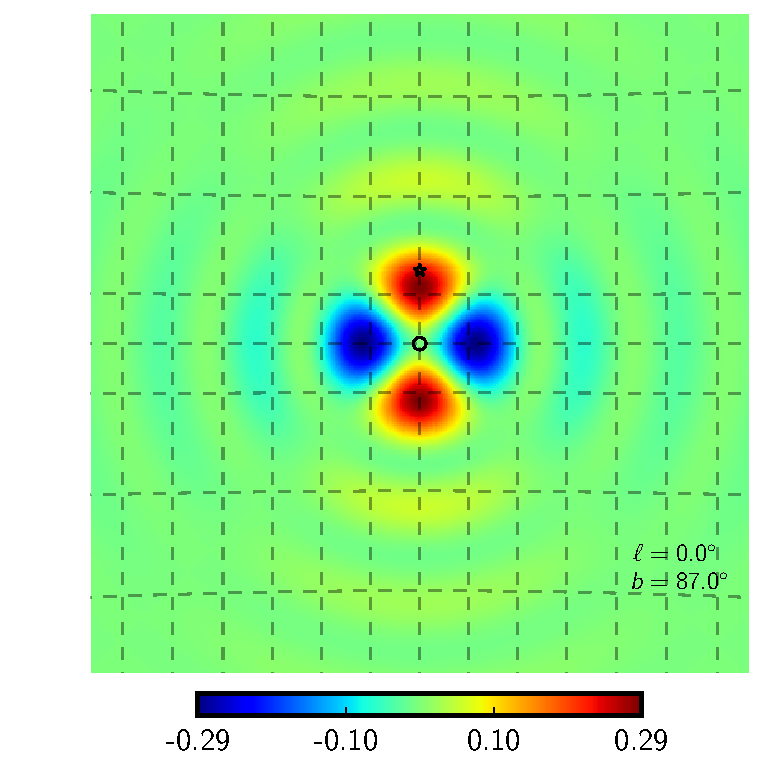
\includegraphics[width=0.16\columnwidth]{kernel/qu2eb_ker_r_lat87_lon0.pdf}}\hspace{-2mm}
\subfigure{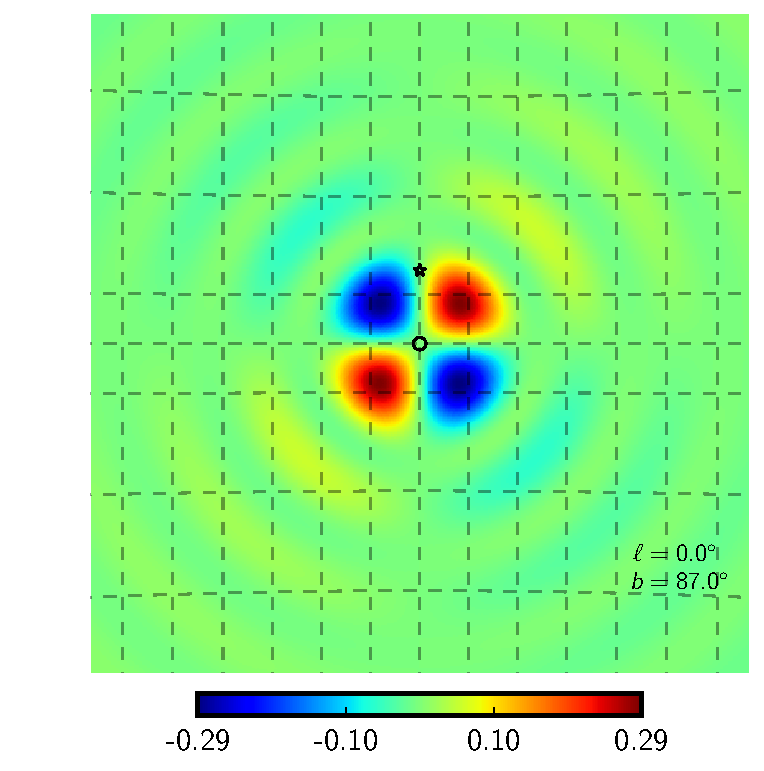
\includegraphics[width=0.16\columnwidth]{kernel/qu2eb_ker_i_lat87_lon0.pdf}}\hspace{-2mm}
\subfigure{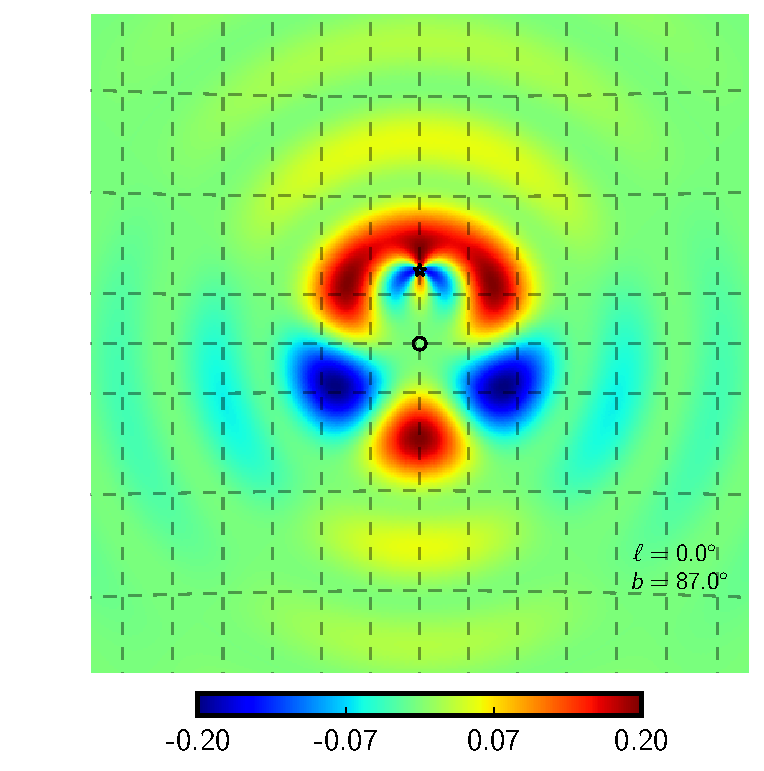
\includegraphics[width=0.16\columnwidth]{kernel/qu2ebqu_ker_r_lat87_lon0.pdf}}\hspace{-2mm}
\subfigure{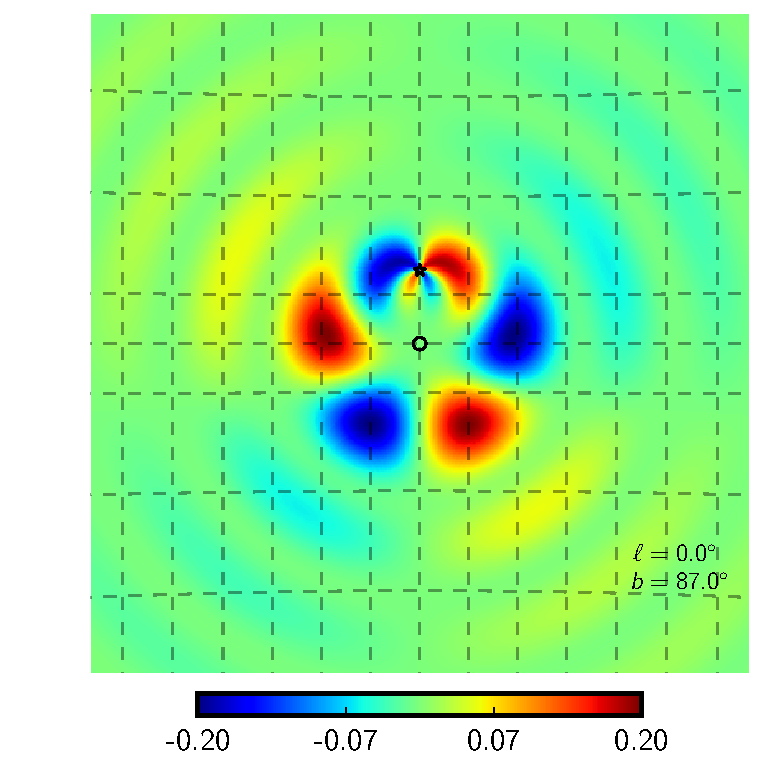
\includegraphics[width=0.16\columnwidth]{kernel/qu2ebqu_ker_i_lat87_lon0.pdf}}\hspace{-2mm}
\subfigure{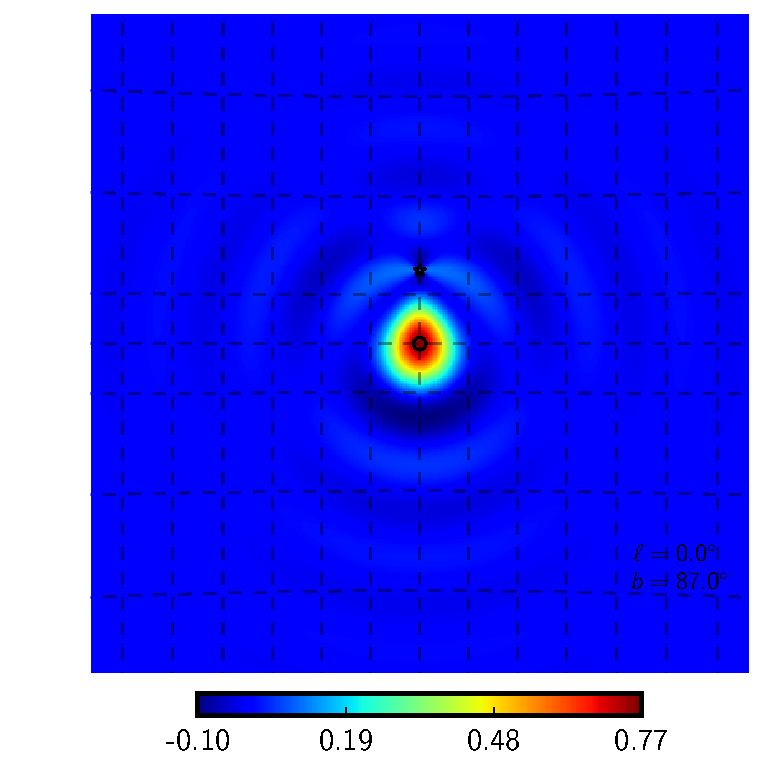
\includegraphics[width=0.16\columnwidth]{kernel/I_ker_r_lat87_lon0.pdf}}\hspace{-2mm}
\subfigure{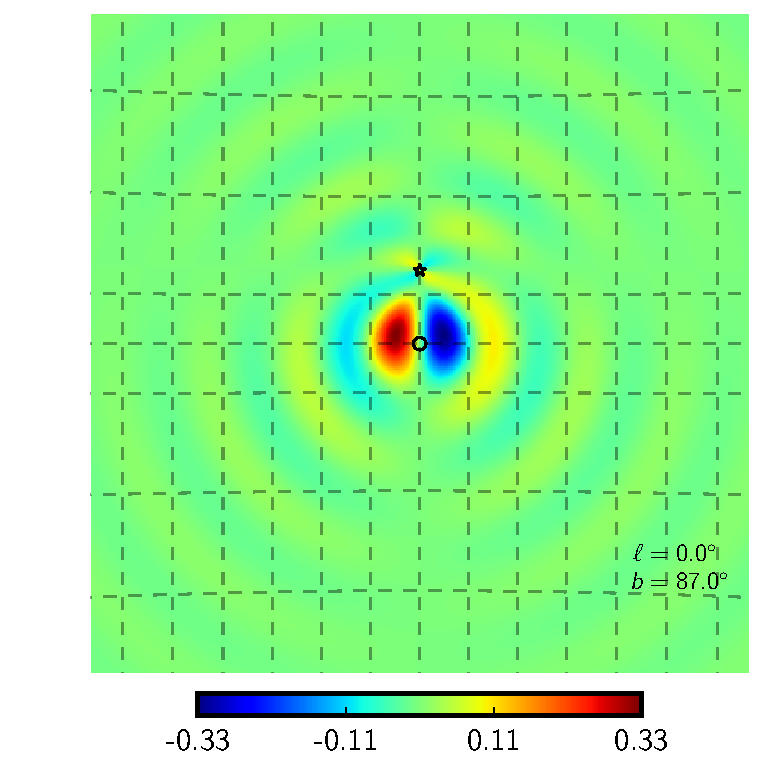
\includegraphics[width=0.16\columnwidth]{kernel/I_ker_i_lat87_lon0.pdf}}\\[-2ex]
\subfigure{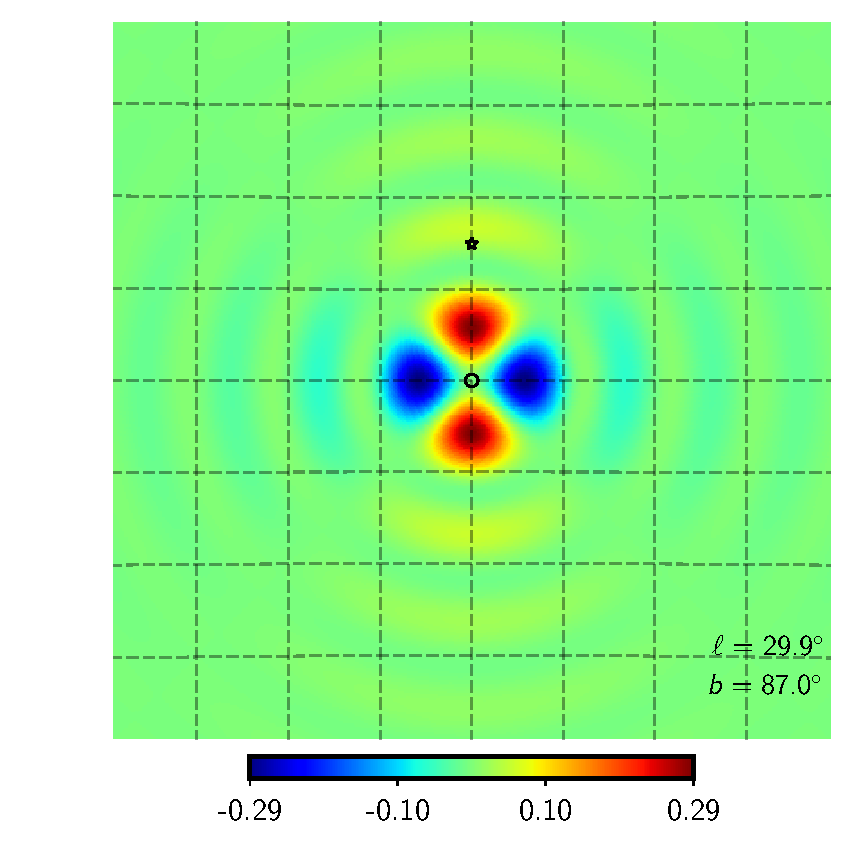
\includegraphics[width=0.16\columnwidth]{kernel/qu2eb_ker_r_lat87_lon30.pdf}}\hspace{-2mm}
\subfigure{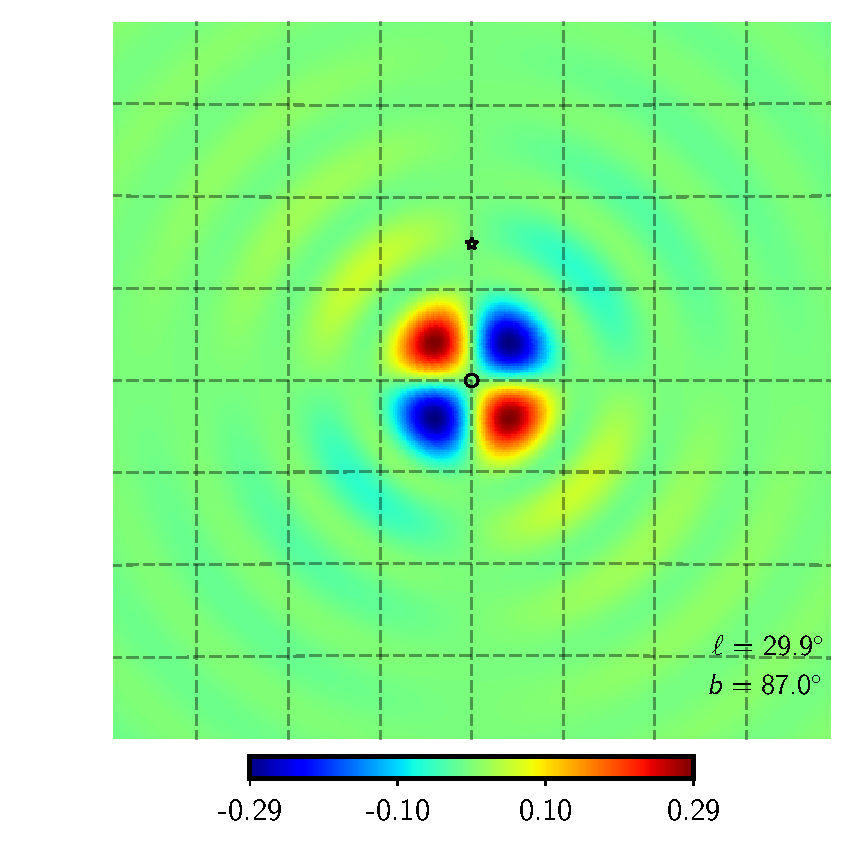
\includegraphics[width=0.16\columnwidth]{kernel/qu2eb_ker_i_lat87_lon30.pdf}}\hspace{-2mm}
\subfigure{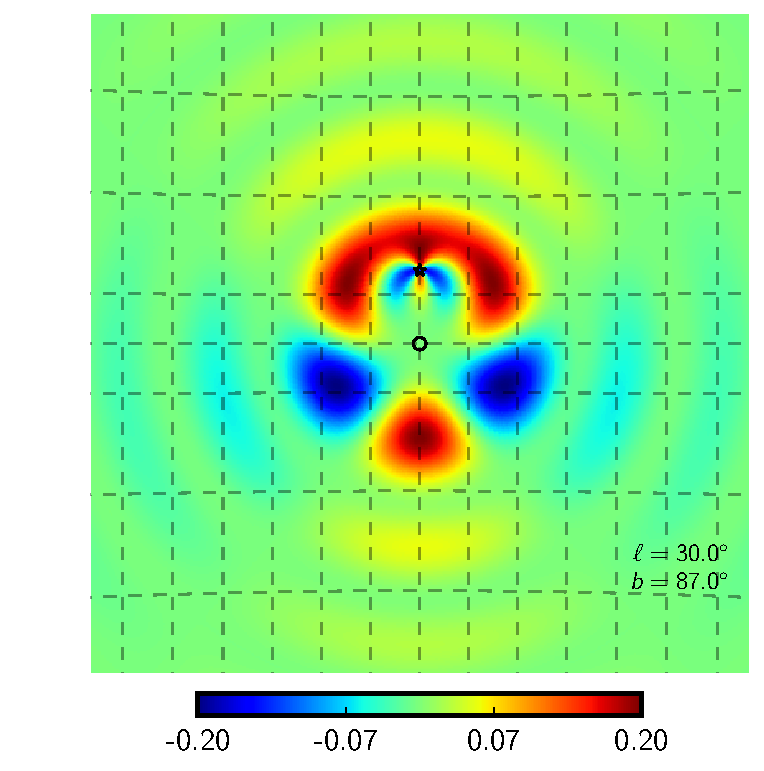
\includegraphics[width=0.16\columnwidth]{kernel/qu2ebqu_ker_r_lat87_lon30.pdf}}\hspace{-2mm}
\subfigure{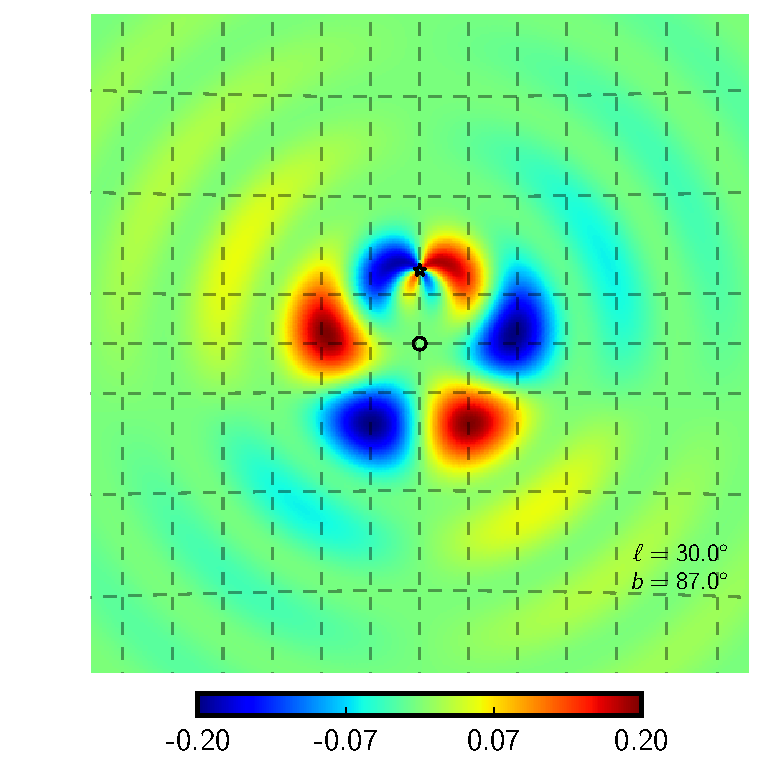
\includegraphics[width=0.16\columnwidth]{kernel/qu2ebqu_ker_i_lat87_lon30.pdf}}\hspace{-2mm}
\subfigure{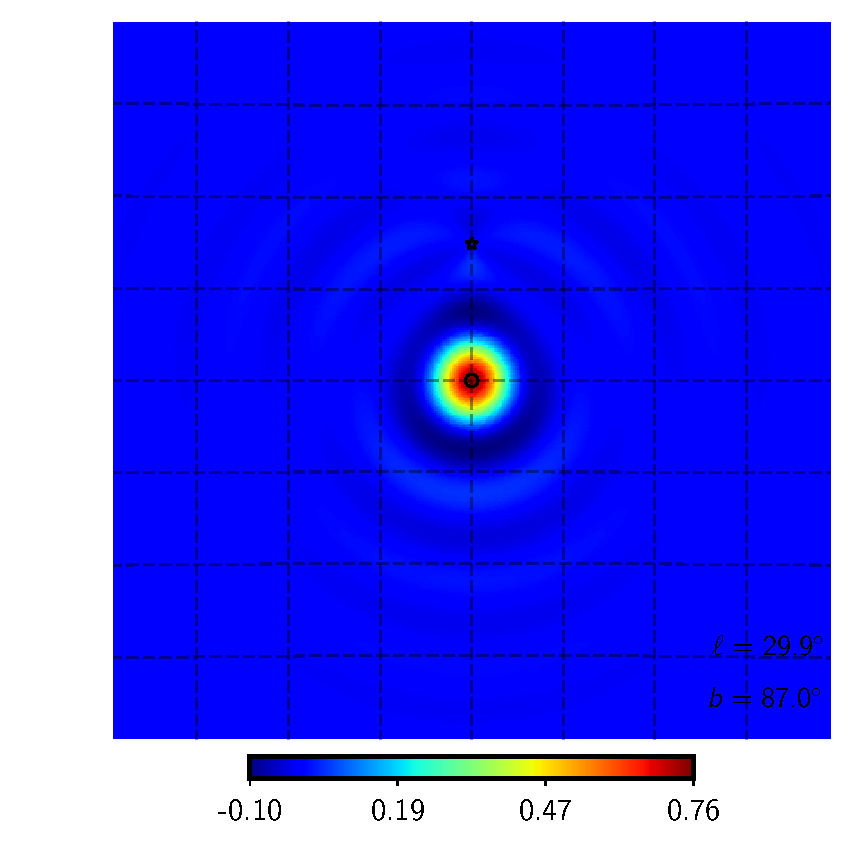
\includegraphics[width=0.16\columnwidth]{kernel/I_ker_r_lat87_lon30.pdf}}\hspace{-2mm}
\subfigure{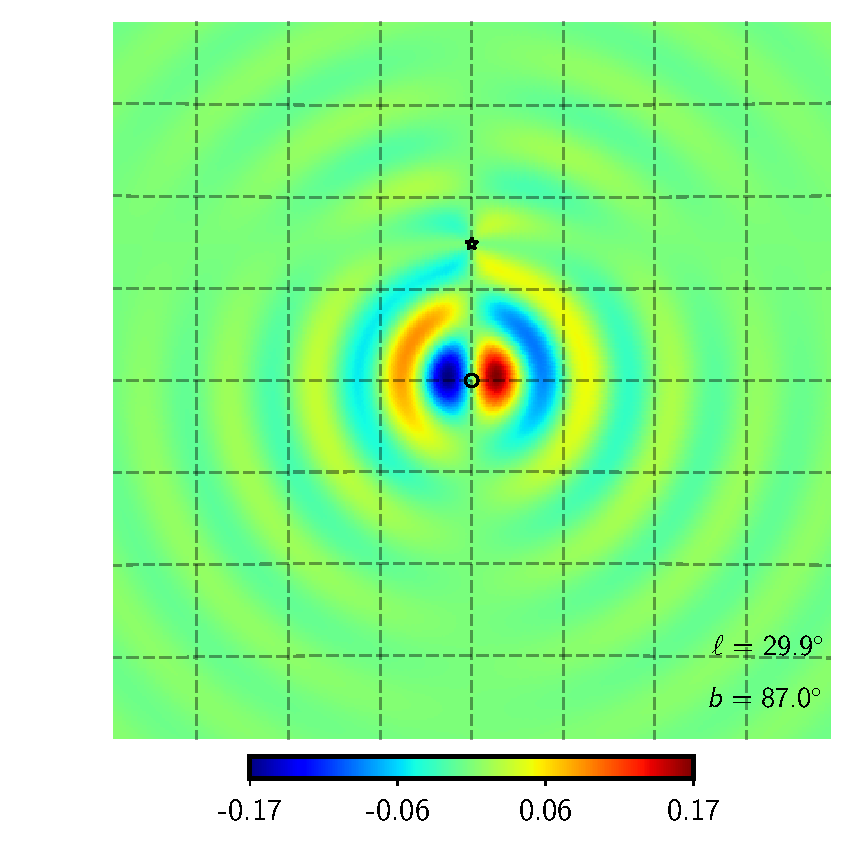
\includegraphics[width=0.16\columnwidth]{kernel/I_ker_i_lat87_lon30.pdf}}\\[-2ex]
\subfigure{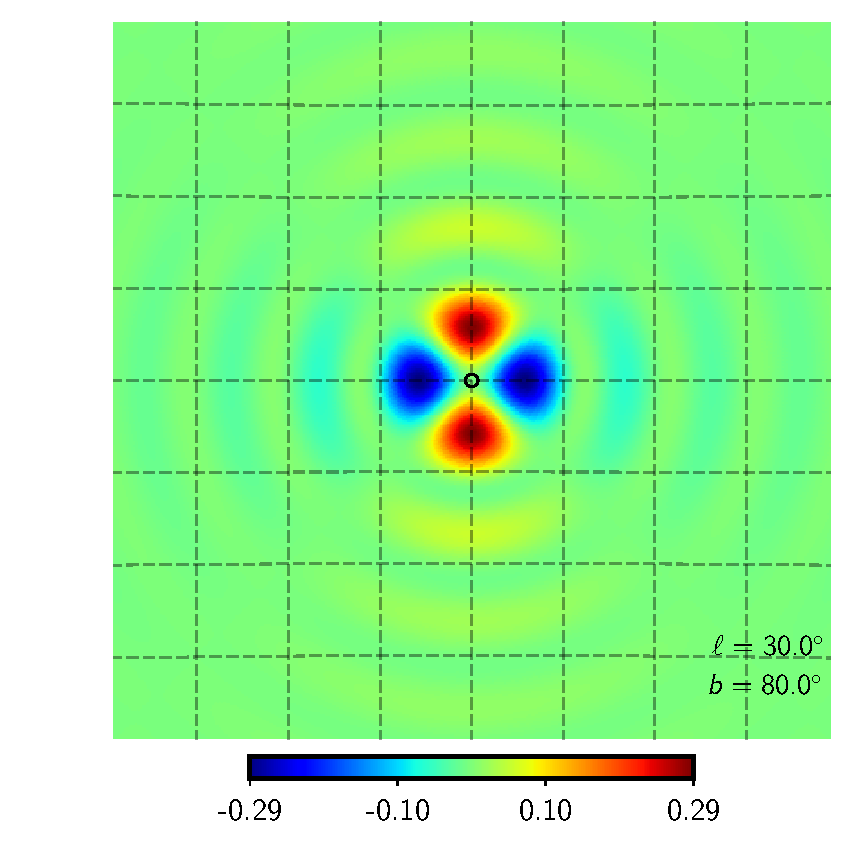
\includegraphics[width=0.16\columnwidth]{kernel/qu2eb_ker_r_lat80_lon30.pdf}}\hspace{-2mm}
\subfigure{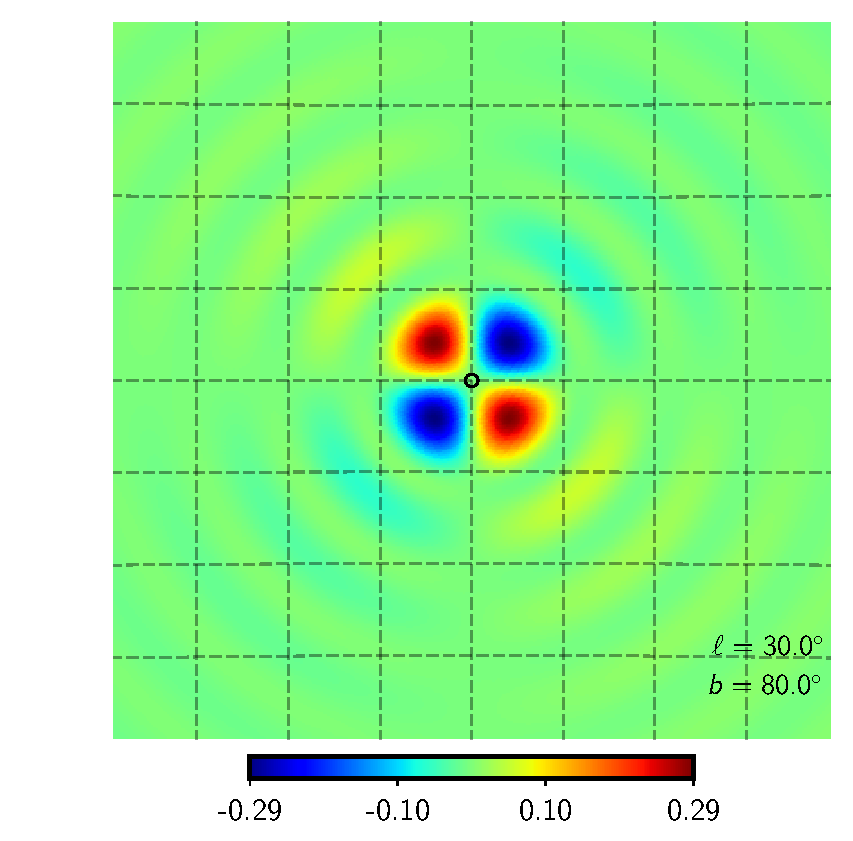
\includegraphics[width=0.16\columnwidth]{kernel/qu2eb_ker_i_lat80_lon30.pdf}}\hspace{-2mm}
\subfigure{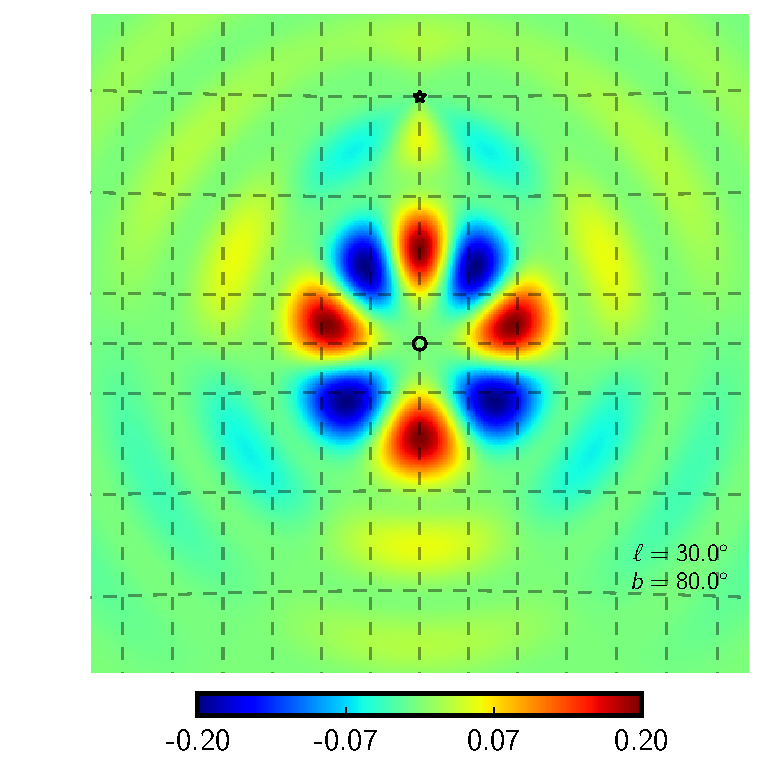
\includegraphics[width=0.16\columnwidth]{kernel/qu2ebqu_ker_r_lat80_lon30.pdf}}\hspace{-2mm}
\subfigure{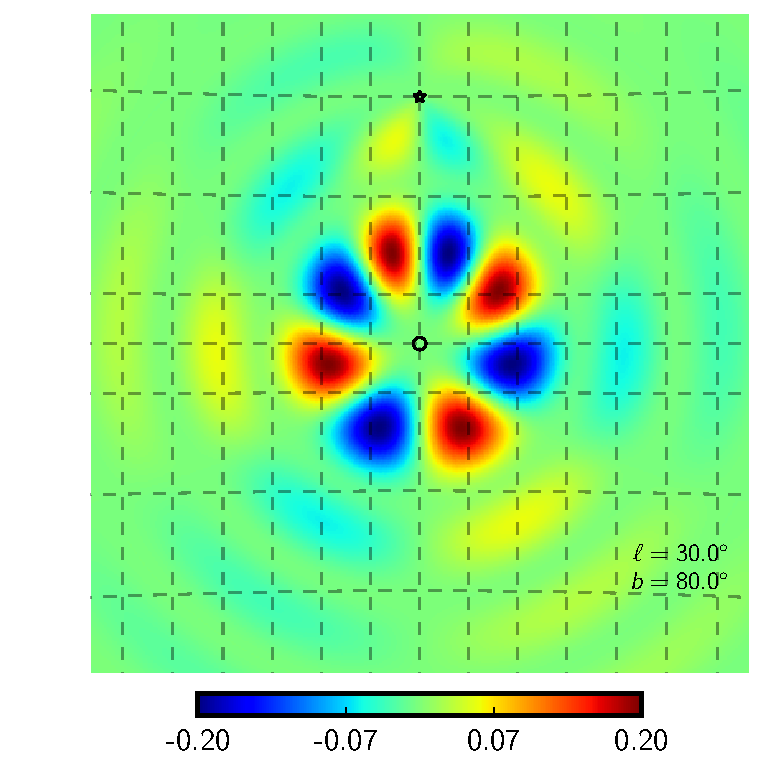
\includegraphics[width=0.16\columnwidth]{kernel/qu2ebqu_ker_i_lat80_lon30.pdf}}\hspace{-2mm}
\subfigure{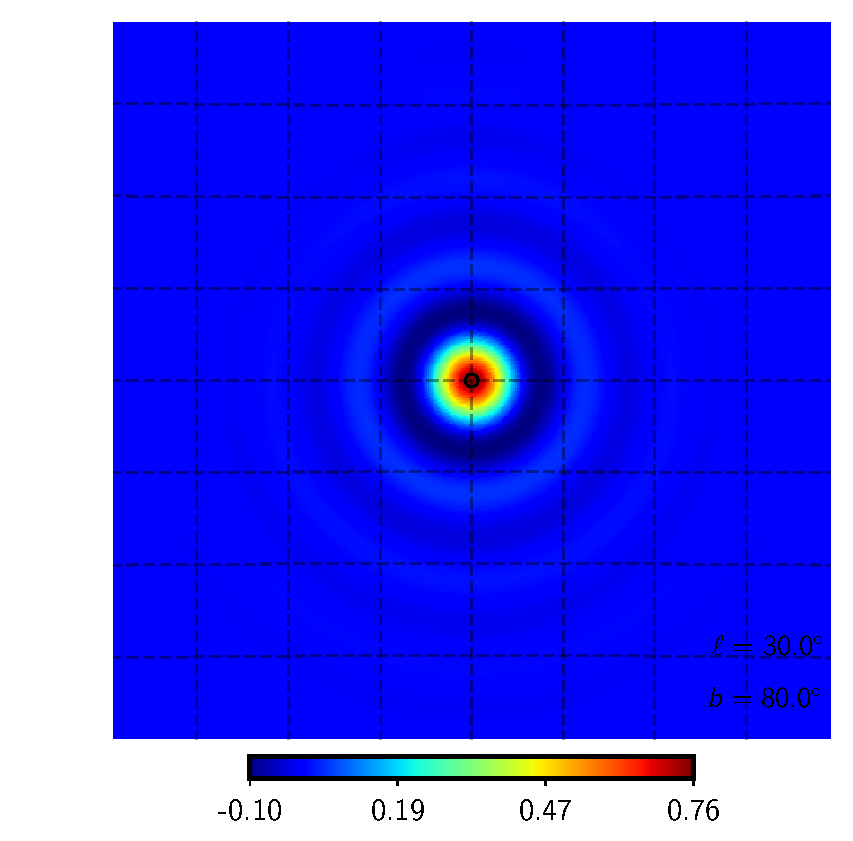
\includegraphics[width=0.16\columnwidth]{kernel/I_ker_r_lat80_lon30.pdf}}\hspace{-2mm}
\subfigure{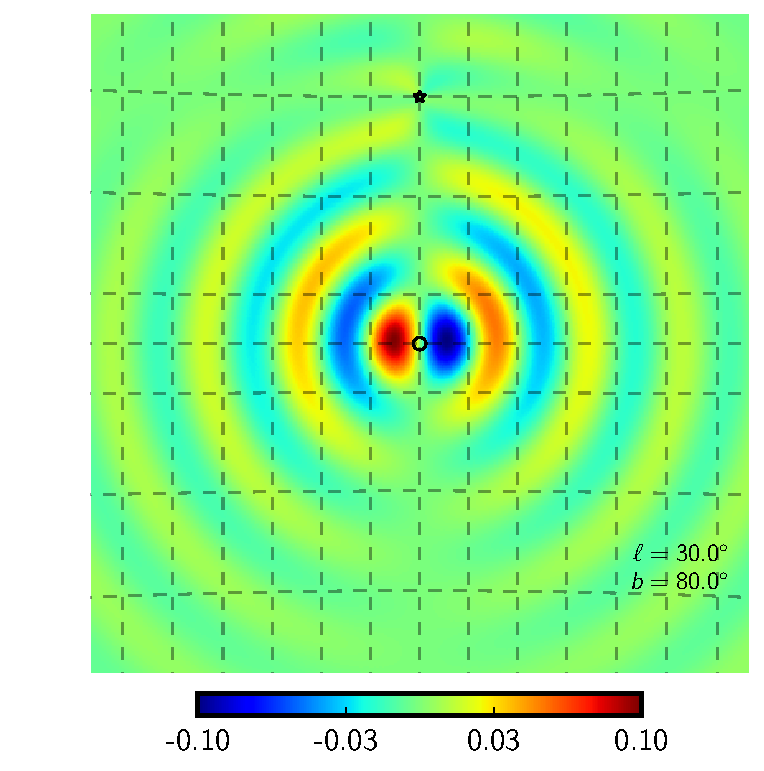
\includegraphics[width=0.16\columnwidth]{kernel/I_ker_i_lat80_lon30.pdf}}\\[-2ex]
\subfigure[$\mathcal{M}_r$]{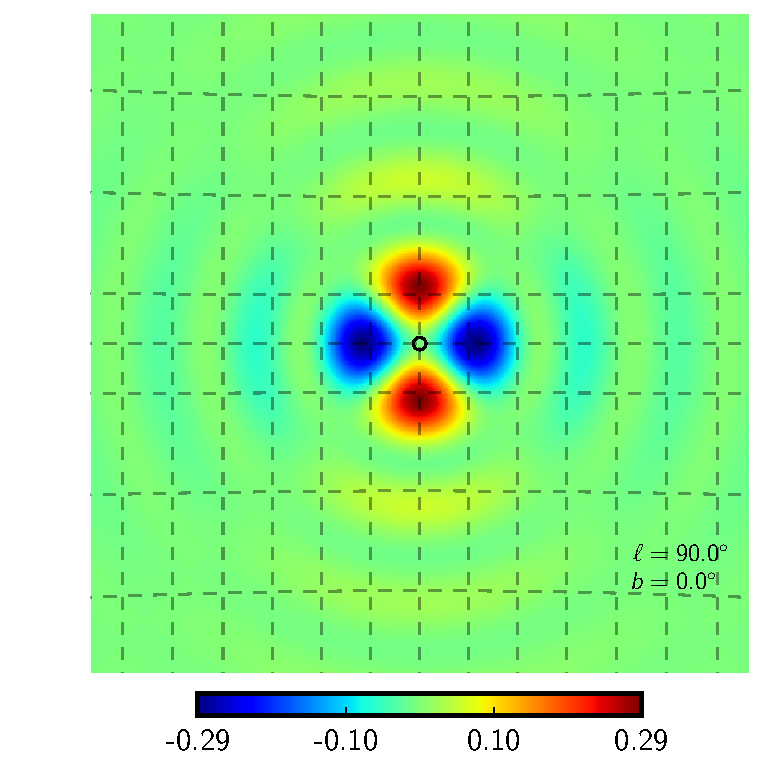
\includegraphics[width=0.16\columnwidth]{kernel/qu2eb_ker_r_lat0_lon90.pdf}}\hspace{-2mm}
\subfigure[$\mathcal{M}_i$]{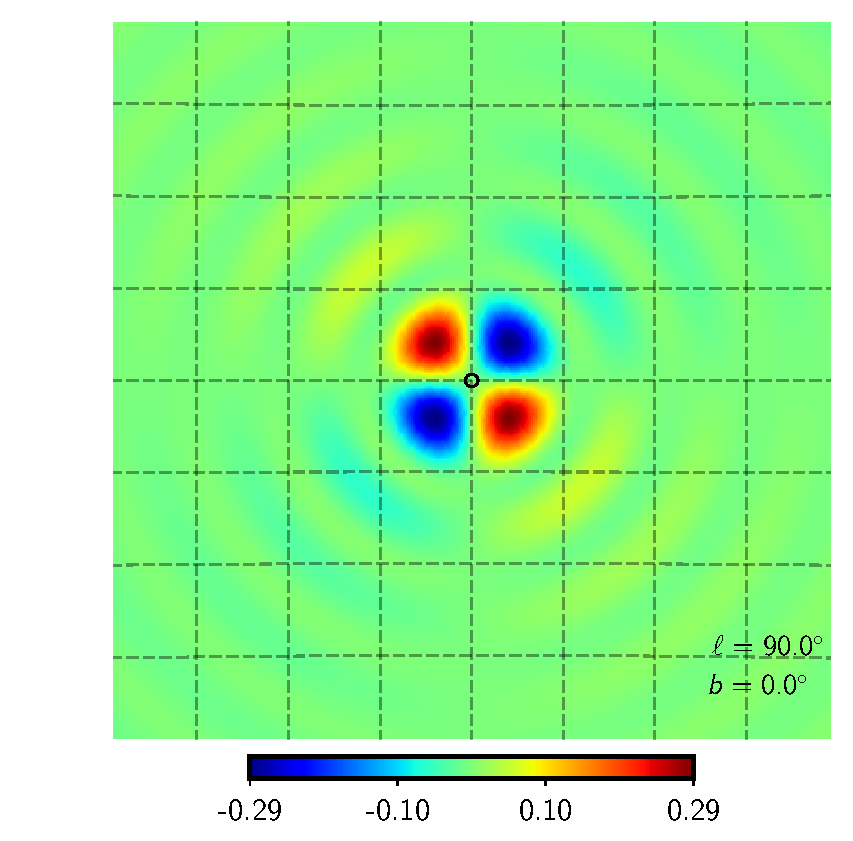
\includegraphics[width=0.16\columnwidth]{kernel/qu2eb_ker_i_lat0_lon90.pdf}}\hspace{-2mm}
\subfigure[$\mathcal{D}_r$]{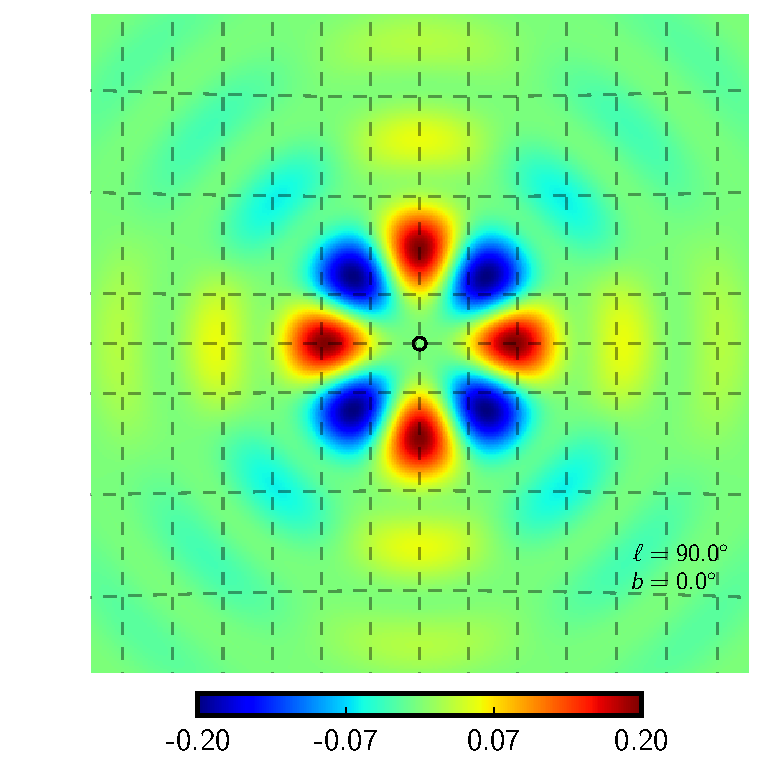
\includegraphics[width=0.16\columnwidth]{kernel/qu2ebqu_ker_r_lat0_lon90.pdf}}\hspace{-2mm}
\subfigure[$\mathcal{D}_i$]{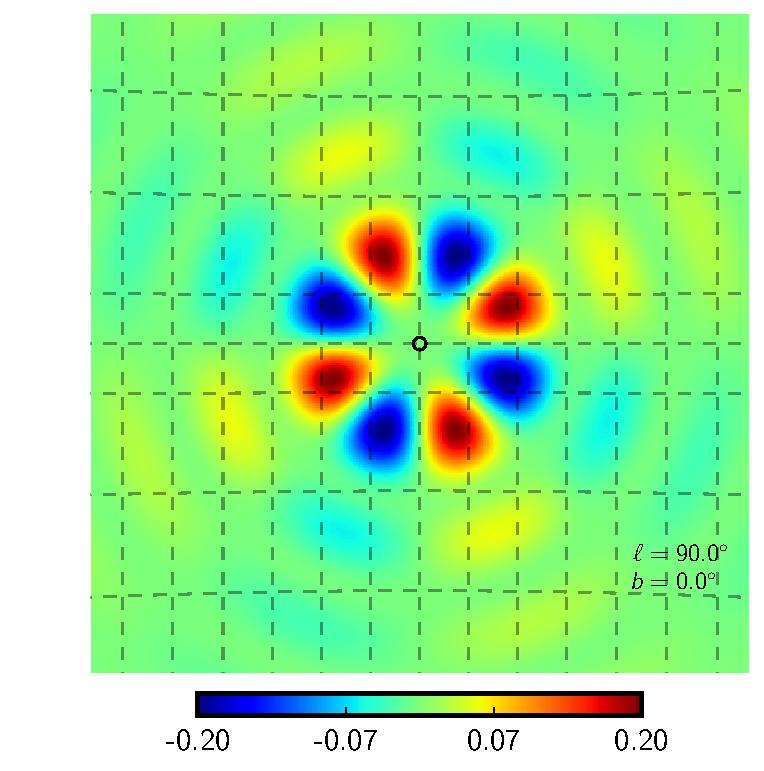
\includegraphics[width=0.16\columnwidth]{kernel/qu2ebqu_ker_i_lat0_lon90.pdf}}\hspace{-2mm}
\subfigure[$\mathcal{I}_r$]{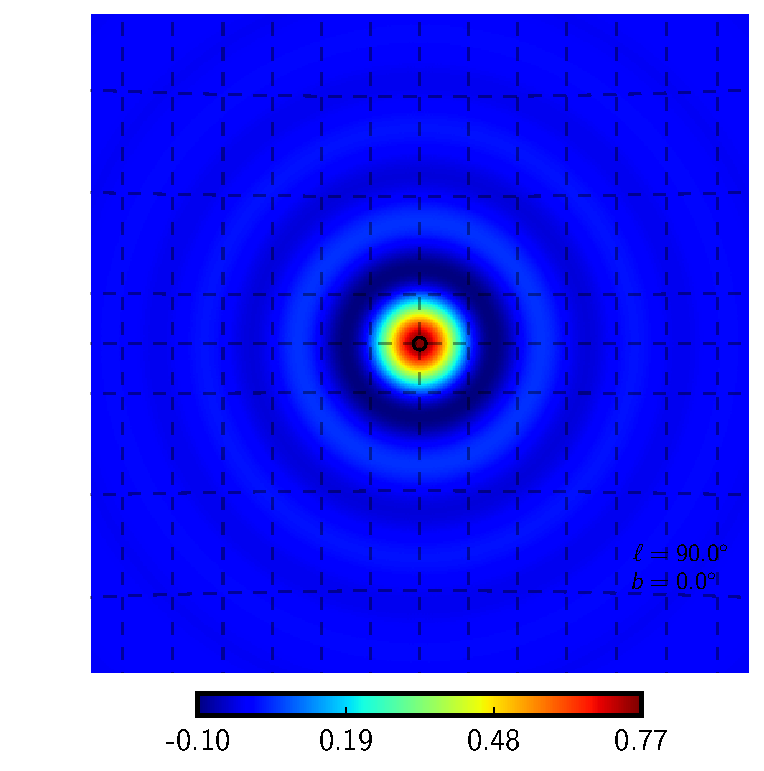
\includegraphics[width=0.16\columnwidth]{kernel/I_ker_r_lat0_lon90.pdf}}\hspace{-2mm}
\subfigure[$\mathcal{I}_i$]{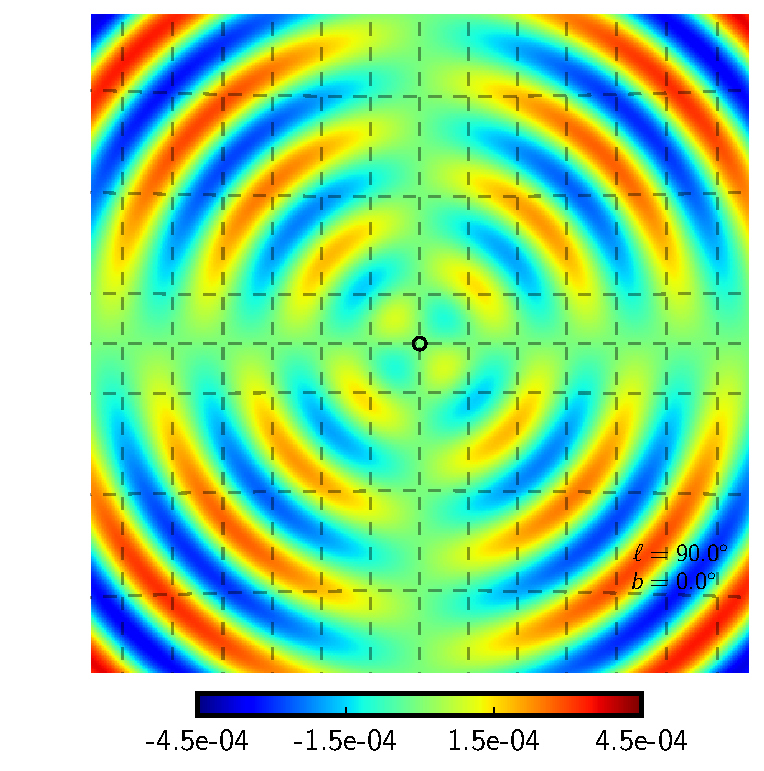
\includegraphics[width=0.16\columnwidth]{kernel/I_ker_i_lat0_lon90.pdf}}
\caption{This panel of figure depicts the various parts of the convolution kernel, discussed in \sec{sec:real_space_operators}. These kernels have been evaluated with the band limit fixed at $\ell_{\rm max}=96$, however the functions have been sampled at an NSIDE=2048 resolution for visual appeal. The size of each panel is approximately $26^{\circ} \times 26^{\circ}$. The black circles denotes the position of the central pixel around which the convolution kernels have been evaluated and the black star marks the location of the north galactic pole. The five rows depict the kernels at different location on the sphere and the galactic coordinates of the central pixel from top to bottom rows are as follows $[b,\ell] = [0^{\circ},0^{\circ}], [87^{\circ},0^{\circ}], [87^{\circ},30^{\circ}], [80^{\circ},30^{\circ}], [0^{\circ},90^{\circ}]$.}
\label{fig:vis_kernel}
 \end{figure}
%
\revisit{Since its not easy to imagine how the Euler angles vary as a function of position of the central pixel, we evaluate and depict the kernel at different locations on the sphere, to give a sense of how these kernels vary across the sphere.}
The function $\mathcal{M}$ is nearly identical irrespective of changes in the galactic latitude and longitude of the central pixel. The only contrasting locations are the poles (i.e. $|b|=90^{\circ}$), where the functions $\mathcal{M}_r$ \& $\mathcal{M}_i$ are rotated by $45^{\circ}$  as compared to the respective functions evaluated at locations where $|b|\neq 90^{\circ}$. It is also important to note that these functions are not distorted when a part of the domain overlaps with the poles, as can be seen in the first four rows of \fig{fig:vis_kernel}. On the contrary, the function $\mathcal{D}$ varies significantly as a function of galactic latitude of the central pixel. It varies from having a two fold symmetry at the poles to having a four fold symmetry at the equator as seen in the middle two columns of \fig{fig:vis_kernel}. This transformation arises from the distortions induced in this function as parts of its domain passes the galactic poles.  The function $\mathcal{I}$ shows similar behavior, varying with latitude and being distorted in parts that overlap with the galactic poles. \revisit{This function, in the ideal case of no band limit would reduces to a delta function at the position of the central pixel ($\lim_{\ell_{\rm max} \to \infty}: \mathcal{I}_r \rightarrow \delta(\hat{n}_0 - \hat{n}'),~ \mathcal{I}_i \rightarrow 0$), \revisit{hints of which can be seen by comparing the amplitudes of the real and imaginary parts of this function in the last two columns of \fig{fig:vis_kernel}, especially close to the equator}. Since we invariably work with a specific band limit, both the real and imaginary parts of this functions make important finite non-zero contributions }. All the function are seen to be invariant under changes in longitude of the central pixel, the latitude being held fixed as can be seen by comparing the figures in the second (evaluated at $[b,\ell]=[87^{\circ},0^{\circ}]$) and third row (evaluated at $[b,\ell]=[87^{\circ},30^{\circ}]$) of \fig{fig:vis_kernel}, as one may have expected.

\subsection{Quantifying the non-locality of E \& B modes} \label{sec:radial_locality}
It is clear that the non-locality of the E and B modes is determined by the radial part of the convolution kernels. To quantify this non-locality as a function of the resolution of the experiment, we evaluate only the radial part of the convolution kernel for different values of the maximum multipole $\ell_{\rm max}$, while keeping the lowest multipole fixed at $\ell_{\rm min}=2$. The set of radial kernels so derived are plotted in \fig{fig:rad_ker_decay}. All the function have been normalized such that their global maxima is set to unity. Note that on increasing $\ell_{\rm max}$ the radial kernels fall appear to shift left, becoming insignificant relative  to their global maxima at progressively small angular distance $\beta$ from the central pixel. 
%
\begin{figure}[!t]
\centering
\subfigure[]{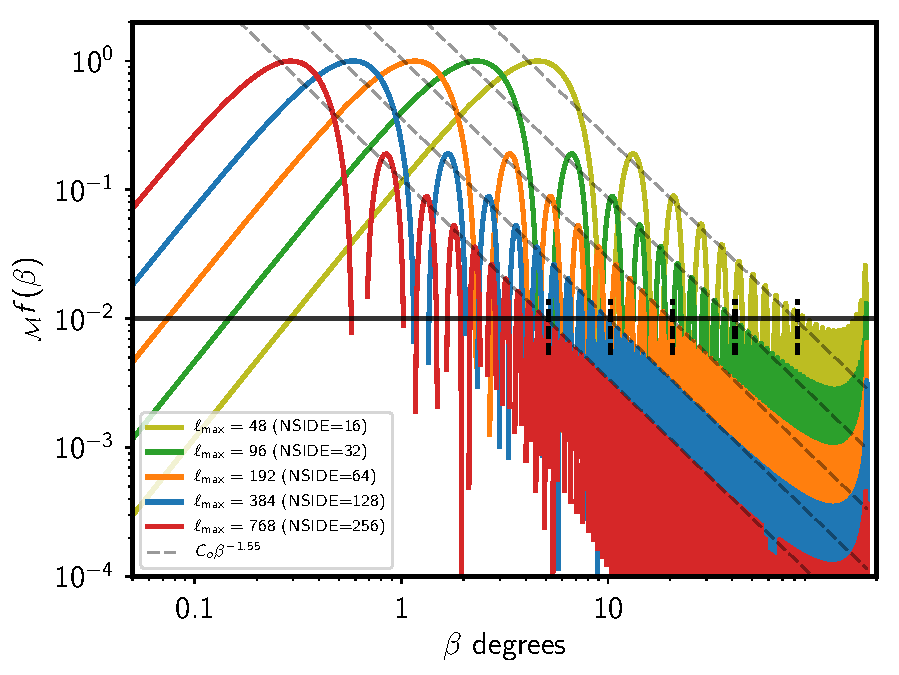
\includegraphics[width=1.0\columnwidth]{kernel/f_rad_ker_fn_of_ellmax.pdf}}
\subfigure[]{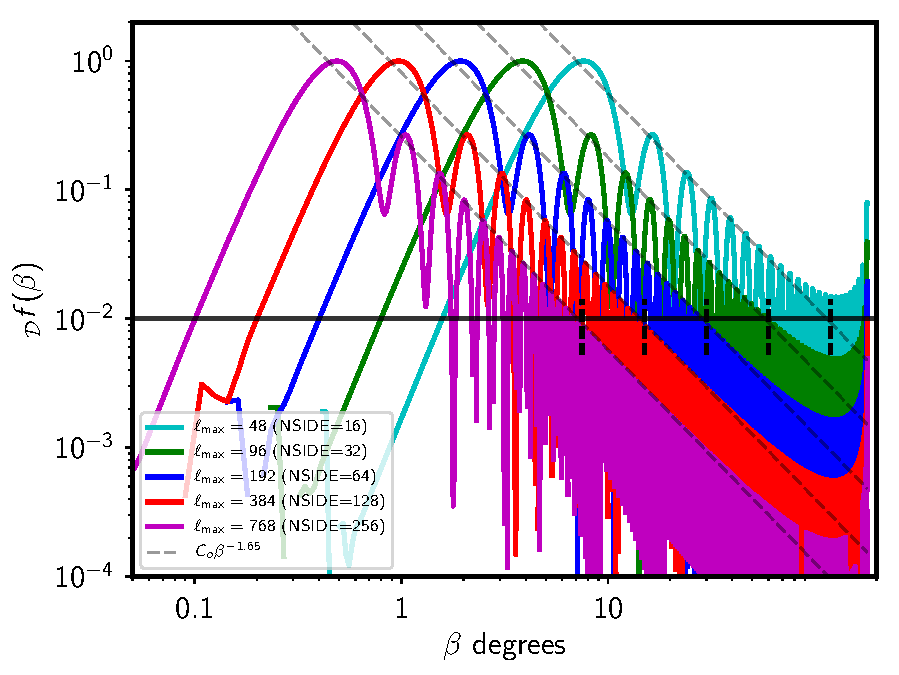
\includegraphics[width=0.48\columnwidth]{kernel/fp2_rad_ker_fn_of_ellmax.pdf}}
\subfigure[]{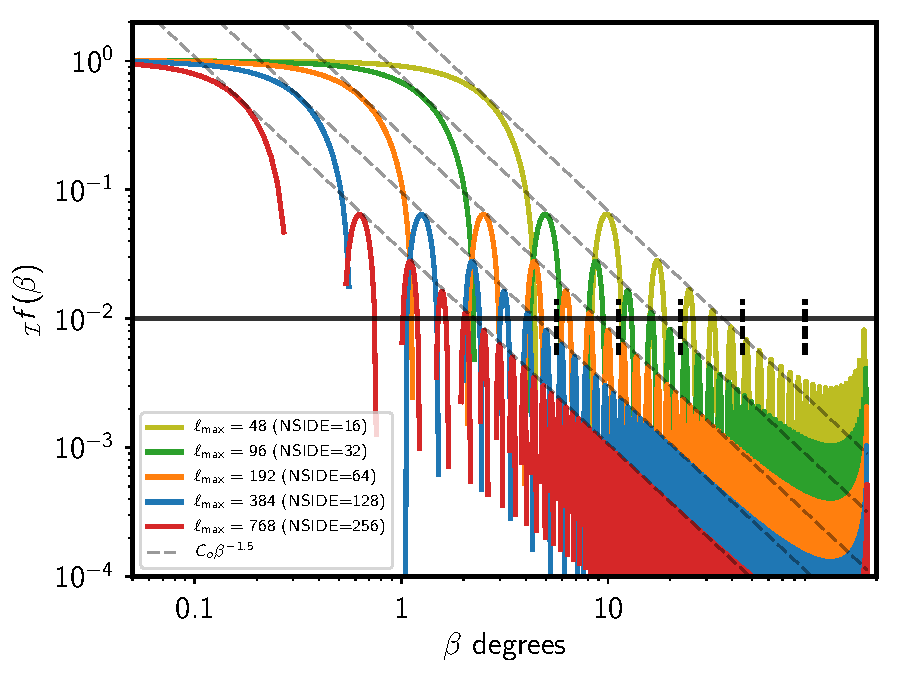
\includegraphics[width=0.48\columnwidth]{kernel/fm2_rad_ker_fn_of_ellmax.pdf}}
\caption{The top panel shows a plot of the radial kernels $f(\beta,\ell_{\rm min},\ell_{\rm max})$ while the bottom left and right panels show the radial functions ${}_{+2}f(\beta,\ell_{\rm min},\ell_{\rm max}) ~\&~ {}_{-2}f(\beta,\ell_{\rm min},\ell_{\rm max})$ respectively, for different $\ell_{\rm max}$ as indicated by the legends and fixed $\ell_{\rm min}=2$. The curves for each of these functions have been normalized such that the maximum of the curve is set to unity. The horizontal solid black line marks the location where the amplitude of the kernel falls below 1\% of its maximum. The slanted dashed black lines indicate a power law fit (by eye) to the envelope of the radial functions. While the envelopes for function $f(\beta)~\&~ {}_{-2}f(\beta)$ are fit well by the power law $\propto \beta^{-1.5}$, the envelope for the function ${}_{-2}f(\beta)$ is seen to have a slightly steeper fall off $\propto \beta^{-1.65}$.}
\label{fig:rad_ker_decay}
\end{figure}
%
We define the value of the abscissa at which the function $f(\beta,\ell_{\rm min},\ell_{\rm max})$ transits to being monotonously below 1\% of the maxima of the function as the non-locality parameter: $\beta_{o}$. We find that the following empirical relation: $\beta_o= {\rm min}(180,180 \frac{24}{\ell_{\rm max}})$ can predict quite accurately the value of the non-locality parameter for a given maximum multipole $\ell_{\rm max}$ and fixed $\ell_{\rm min}=2$. 

The envelope of the radial kernel $f(\beta,\ell_{\rm min},\ell_{\rm max})$ is observed to have a linear relation to the angular distance $\beta$ in log space as seen in \fig{fig:rad_ker_decay}, indicating a power law fall off. A fit by eye indicates that the envelope of the function is well represented by a fuction proportional to $\beta^{-1.5}$ in intermediate angular distance range. This is not valid in regions $\beta << \beta_o$ and $\beta >> \beta_o$, where the envelope of the function can be clearly seen to deviate from power law behavior (see \fig{fig:rad_ker_decay}).

\comment{There isn't too much of a discussion surrounding the function ${}_{\pm}f(\beta)$. What do you want to say about these functions?}

\comment{Do you want to comment on the telescoping behavior of these radial functions ? }
